\subsubsection{Normalized Difference Soundscape Index}
One goal within the field of soundscape ecology is the analysis of the key characteristics of the Anthropocene, that is, the impact that humans have on wildlife and Earth as a whole. And perhaps no other metric of analysis symbolizes this better than the Normalized Difference Soundscape Index (NDSI). NDSI has the goal of measuring the ratio between anthropogenic sounds and biological sounds.\par
The basis of this metric originates from a 2004 thesis written by Brian Michael Napoletano entitled \textit{Measurement, Quantification and Interpretation of Acoustic Signals Within an Ecological Context.} In this paper, Napoletano proposed three classifications for the sources for domains of sound frequencies: geophony (full spectrum), anthrophony (0 to 2 kHz), and biophony (3 to 11 kHz).\cite{napoletano} By ignoring potential geophony (as it would occur over too wide of a spectrum to identify), NDSI measures the acoustic energy (in watts) produced within the anthrophony and biophony spectrums.\par
With these metrics at hand, NDSI can be calculated using the following formula:\par

\begin{equation}
  NDSI = \frac{\beta - \alpha}{\beta + \alpha}
\end{equation} \\[-24pt]

In which \(\beta\) represents the amount of acoustic energy in the biophony domain and \(\alpha\) represents the amount of acoustic energy in the antrophony range. As a result, the NDSI value can range between -1 to represent pure anthrophony and 1 to represent pure biophony within a soundscape over space and time.\cite{gage}\par
Of course, this metric has its limits. In addition to completely ignoring all signals of geophony, NDSI fails to take into account variations in acoustic energy patterns depending on the source of sound, the time of day, and the season. As an example, Figure ~\ref{fig:ndsiGraphs} shows acoustic energy variation in different agricultural environments within different frequency ranges over the course of a day by hour.\par
With these conditions in mind, while NDSI may not be the end-all-be-all for interpreting levels of biophony and anthrophony within a region, it can still be a useful metric, especially when run against a large, representative data set and used alongside other metrics.\par

\begin{figure}
  \begin{center}
    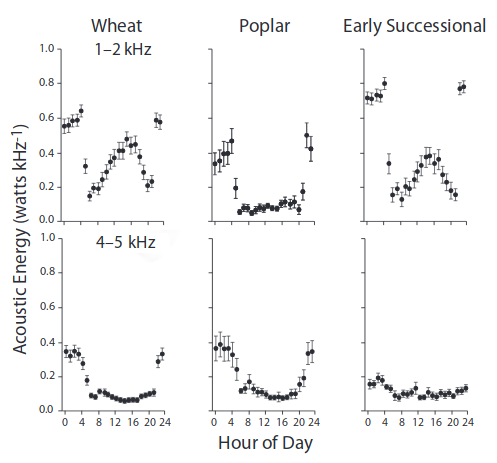
\includegraphics[width=0.7\textwidth]{NdsiGraphs}
  \end{center}
  \caption{Levels of acoustic energy within different environments and different frequency domains}
  \label{fig:ndsiGraphs}
\end{figure}
